%!TEX root = ../CallenThermo.tex

\chapter{可逆过程和最大功定理}\label{chap4}

\section{可能和不可能的过程}\label{sec4.1}

一名工程师常会需要通过设计一个装置来完成某个任务——例如让一个电梯升到高楼上。因此他就得弄出一个联动装置,或者“引擎”,来可控的将能量从火炉里转移到电梯上;{\it 如果}火炉里的热量通过数个活塞、杠杆和凸轮转换成了电梯上升所需要的能量。但谋事在人,成事由“天”(例如,物理定律)%
\mpar{原文为 "But 'nature'(i.e. the law of physics) exercise the crucial decision"}%
——这件事到底是能办成呢,还是设备干脆就停着不动,没有热量从火炉里出来,电梯也没上升一丝一毫。结果得取决于两点。其一是引擎得要满足力学定律(自然包括能量守恒),其二,这个过程必须使熵向着最大增长。

专利局里充满了各路在逻辑上无可挑剔的(如果A发生那么B一定发生)失败发明——这些天才般的设计满足所有力学定律,但依旧固执的停在那儿,默默地拒绝熵的减小。其他的一些能动起来,但会产生一些意料之外的结果,比发明者预料中更有效的使熵增加。

如果,虽然如此,这个网络被在保证总能量不变的前提下最大可行的增加总的熵,那么将不会有什么基本定律来否决掉这样一个恰当的过程的存在。尽管实现这样适当的引擎可能需要相当的天才成分,但它起码在原则上来讲是可行的。

\begin{example}\label{eg4.1}
一个约束系统具有确定摩尔数和体积,则其不能对外界做功。另外,这个系统的热容是常数$C$。则这个系统的基本方程是$S=S_0+C\ln(U/U_0)$,其中$U=CT$。\\
两个具有相同热容量的此类系统,初态分别具有温度$T_{10}$和$T_{20}$,其中$T_{10}<T_{20}$。一个用于升降电梯的引擎(即对一个纯力学系统做功),从这两个热力学系统中获取能量。它们最大能获得多少功?\\
{\bf 求解:}\\
这两个热力学系统最终会达到相同的温度$T_f$。其能量的总改变量为
\[
\Delta U = 2CT_f-C(T_{10}+T_{20})
\]
而力学系统(“电梯”)所获得的功为$W=-\Delta U$,即
\[
W = C(T_{10}+T_{20}-2T_f)
\]
熵的总改变量为两个热力学系统的改变量之和,为
\[
\Delta S = C\ln\frac{T_f}{T_{10}} + C\ln\frac{T_f}{T_{20}} = 2C\ln\frac{T_f}{\sqrt{T_{10}T_{20}}}
\]
为了使$W$最大,我们自然希望$T_f$最小(从第二式容易看出),根据第三式我们知道这意味着要使$\Delta S$取极小。而$\Delta S$最小就只能是零了,对应着一个可逆过程。这样最优的引擎能得到
\[
T_f = \sqrt{T_{10}T_{20}}
\]
和
\[
W = C(T_{10}+T_{20}-2\sqrt{T_{10}T_{20}})
\]
\end{example}

作为补充,我们需要注意到假设两个热力学系统最后到达一个相同的温度是不必要的;$W$可以分别对$T_{1f}$和$T_{2f}$作优化,最后能得到同样的结果。对于末温相同这个简化假设,我们可以用自洽性来论证:如果末温不同,那么我们可以通过这个办法来继续获取更多的能量。

\begin{example}
例\ref{eg4.1}的一个有趣的变体是三物体(每一个都是例\ref{eg4.1}中描述的类型,有$U=CT$)初始温度分别为\SI{300}{\kelvin}、\SI{350}{\kelvin}、\SI{400}{\kelvin}。其需求是尽可能高的提高{\it 一个}物体的温度,而不论其他两个物体怎么样(并且不改变任何外部系统的状态)。那么这里一个物体最高能到多高温度?\\
{\bf 求解:}\\
将三个初始温度用$T_1$,$T_2$,$T_3$标记,单位取作\SI{100}{\kelvin}($T_1=3$,$T_2=3.5$以及$T_3=4$)。类似的,令单个物体能达到的最高温度记做$T_h$。可以推断剩下两个物体的末温{\it 都}是$T_c$(否则,我们可以用例\ref{eg4.1}的办法来对外做功,然后将功转换为热物体上的热)。能量守恒要求
\[
T_h + 2T_c = T_1 + T_2 + T_3 = 10.5
\]
总的熵增为
\[
\Delta S = C\ln\frac{T_c^2T_h}{T_1T_2T_3}
\]
熵增为正要求
\[
T_c^2T_h \ge T_1T_2T_3 \quad (=42)
\]
利用能量守恒式消去$T_c$
\[
(5.25-\frac{T_h}{2})^2T_h\ge 42
\]
方程左端对$T_h$作图。绘图范围从$0$到$10.5$,上界是为了保证$T_c$为正。图像表明使纵坐标大于$42$的最大$T_h$值是
\[
T_h = 4.095 \quad(\text{或}T_h = \SI{409.5}{\kelvin})
\]
这个值使不等式取等,即对应可逆过程。
\end{example}

这道题的另一个解法见习题4.6-7。

\ 

{
	\centering
	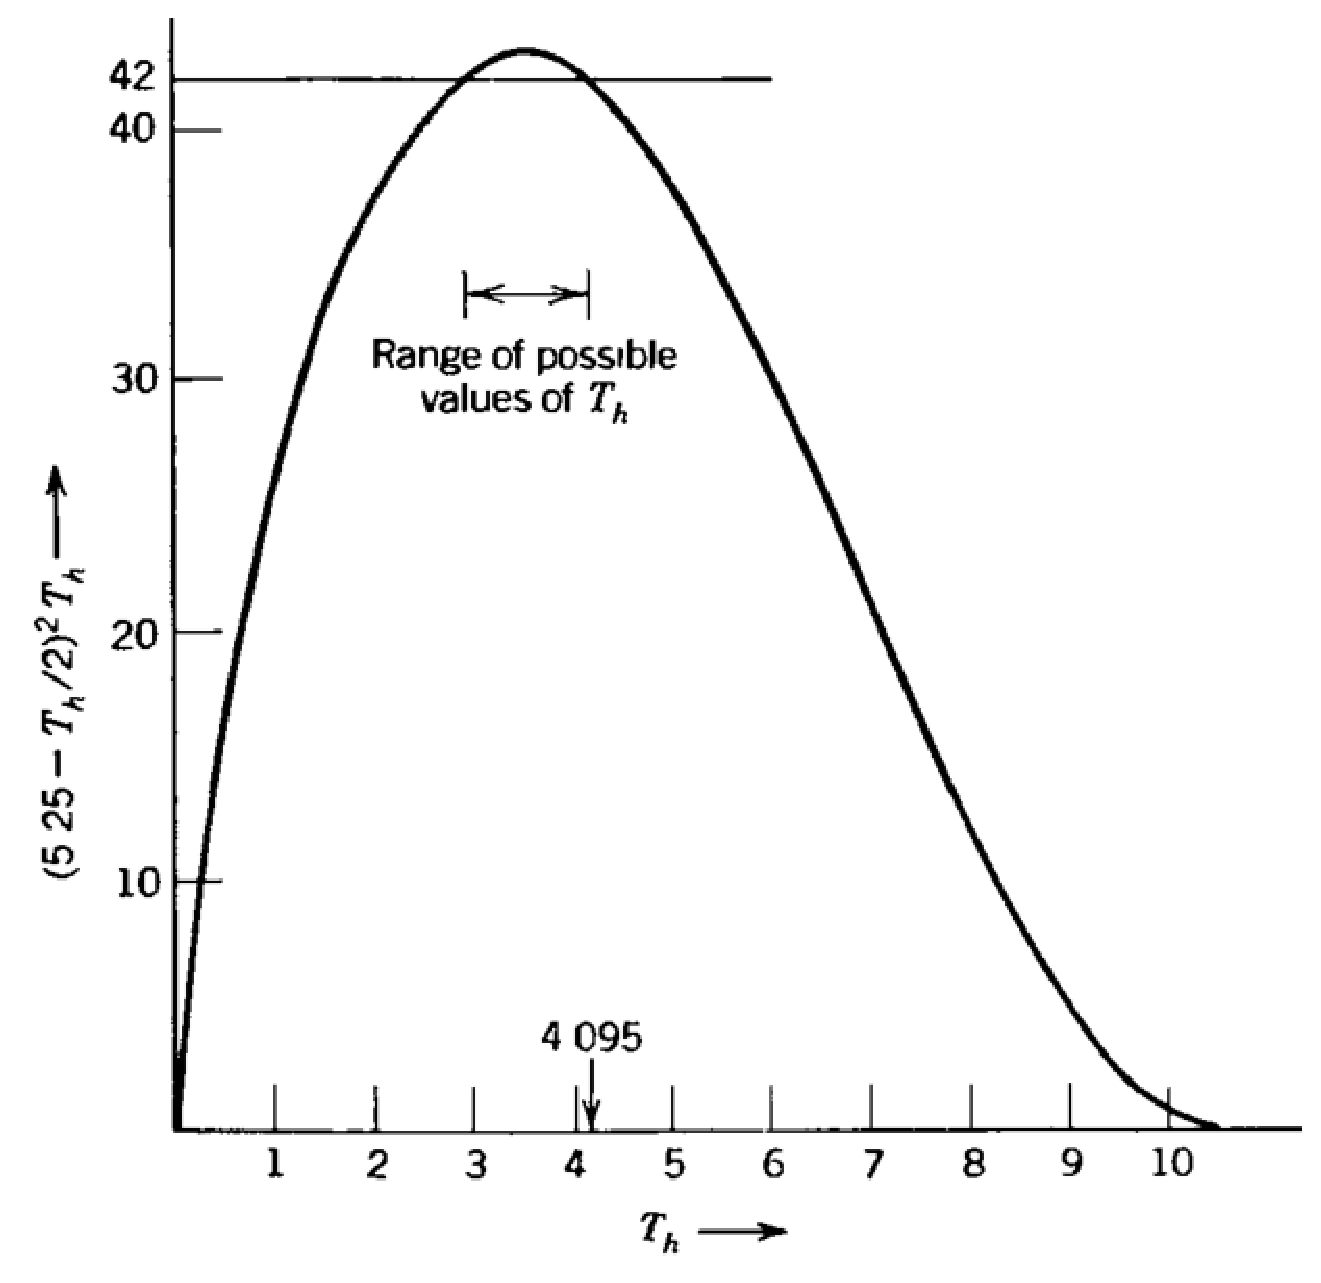
\includegraphics[scale=0.5]{fig4_01.eps} 
	\figcaption{ }
}

\subsection*{习题}
\begin{itemize}
\item[4.1-1.] 一摩尔单原子理想气体和一摩尔$c=3/2$的理想 van der Waals 流体(\ref{sec3.5}节)分别装在体积为$v_1$和$v_2$的容器里。理想气体的温度为$T_1$而 van der Waals 流体是$T_2$。我们希望将理想气体的温度变成$T_2$而保持总的能量不变。那么 van der Waals 流体的末温是多少?各参数($T_1,T_2,a,b,v_1,v_2$)之间需要满足什么关系才能实现这样一个温度转换(总是假定在过程中外界不发生改变)?
\item[4.1-2.] 一个橡胶带(\ref{sec3.7}节)初始温度为$T_B$,长度为$L_{B}$。一摩尔单原子理想气体初温为$T_G$,体积为$V_G$。理想气体经历一个定容升温过程达到温度$T_G'$。其所需要的能量全都从橡胶带中获得。那么橡胶带的长度是否需要改变?如果是的话,改变多少?
\begin{flushright}
{\it 答案:}\\
若$l=L_B-L_0$,
\[
l^2-(l')^2\ge 2b^{-1}cL_0(L_1-L_0)\ln\left(1-\frac{3R}{2RL_0}\frac{T_G'-T_G}{T_B}\right)+3Rb^{-1}(L_1-L_0)\ln(T_G'/T_G)
\]
\end{flushright}
\item[4.1-3.] 假设例\ref{eg4.1}中的两个系统热容具有形式$C(T)=DT^n$,其中$n>0$:\\
\begin{enumerate}
\item 证明这样的系统内能$U=U_0+DT^{n+1}/(n+1)$以及熵$S=S_0+DT^n/n$。系统的基本方程是什么?
\item 如果其初始温度分别为$T_{10}$和$T_{20}$,最大可输出功为多少(两系统最后处于相同温度)?
\end{enumerate}
\begin{flushright}
{\it 答案:}\\
对于$n=2$:
\[
W=\frac{D}{3}\left[T_{10}^3+T_{20}^3-\frac{1}{\sqrt{2}}(T_{10}^2+T_{20}^2)^{3/2}\right]
\]
\end{flushright}
\end{itemize}

\section{准静态和绝热过程}\label{sec4.2}
熵极大作为中心原理,当应用于不同类型的过程时能给出不同的定理。我们先重新给出对状态和过程的概念的描述,然后再来关注这些定理。

为了描述一个热力学状态的特征及其可能的过程,{\it 热力学构形空间(thermodynamics configuration space)}的引入将是有必要的。一个简单系统的热力学构形空间是由熵和诸广延量$U, V, N_1,\dots ,N_r$坐标轴张成的抽象空间。系统的基本方程$S=S(U, V, N_1,\dots ,N_r)$在r热力学构形空间中定义了一个曲面,如图\ref{fig4.1}所示。另外注意图\ref{fig4.1}与$(\partial U/\partial S)_{\dots , X_j,\dots}(\equiv 1/T)$为正,以及$U$是$S_{\dots , X_j,\dots}$的单值函数的要求相符。
\begin{figure}
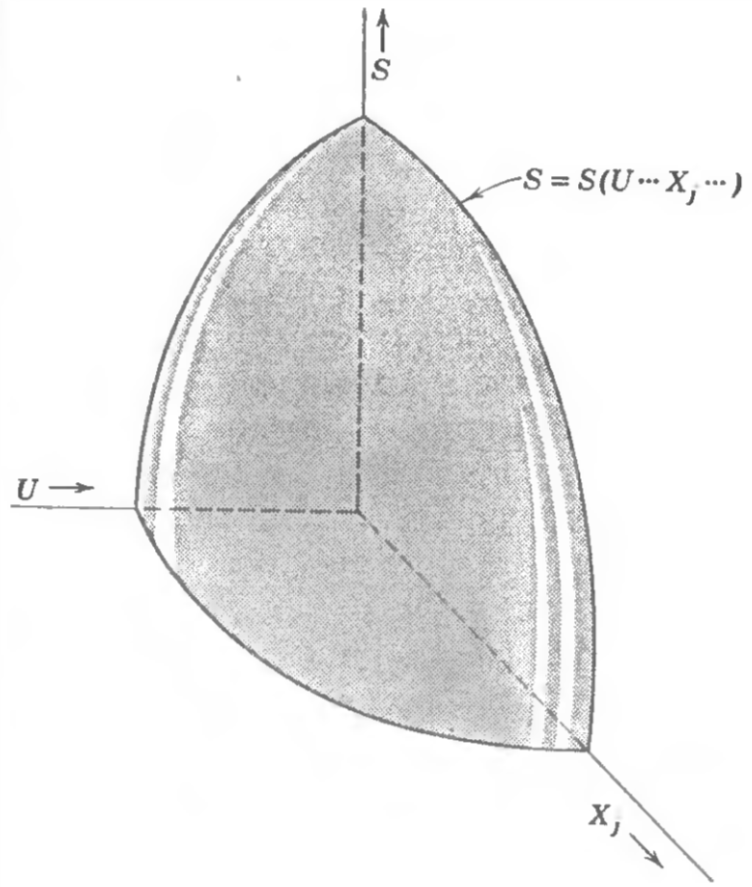
\includegraphics[width=.8\textwidth]{Pictures/fig4.1.png}
\figcaption{一个简单系统的热力学构形空间中的超曲面$S=S(U, \dots, X_j,\dots)$。}
\label{fig4.1}
\end{figure}
根据定义,构形空间中的每一个点代表一个平衡态。而非平衡态需要一个维度大得多的空间中的点来表示。

一个复合体系的基本方程可以由包括了全部子系统的广延量的构形空间中的一张曲面。对于含有两个子系统的复合系统,其构形空间的坐标轴应该包括总熵$S$和两个子系统的广延量。一个更方面的选择是总的熵$S$、第一个子系统的广延量$(U^{(1)},V^{(1)},N^{(1)}_1,N^{(1)}_2,\dots)$、以及整个复合系统的广延量$(U,V,N_1,N_2,\dots)$。复合系统构形空间的一个示例见图\ref{fig4.2}。

\begin{figure}
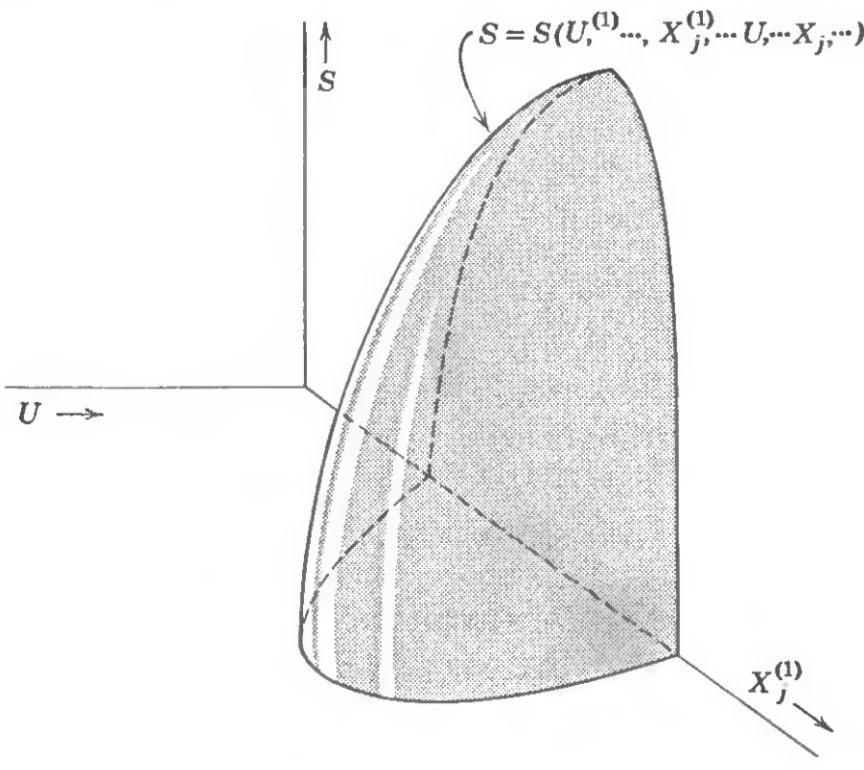
\includegraphics[width=.8\textwidth]{Pictures/fig4.2.png}
\caption{一个复合系统的热力学构形空间中的超曲面$S=S(U^{(1)}, \dots, X^{(1)}_j,\dots,U, \dots, X_j,\dots)$。}
\label{fig4.2}
\end{figure}

考虑超曲面上任意一条从初态到末态的曲线,如图 。这样的曲线被称为{\it 准静态轨迹(quasi-static locus)}或{\it 准静态过程(quasi-static process)}。一个准静态过程可以由一连串密集的{\it 平衡}态来定义。值得强调的是,准静态过程是一个理想的概念,而实际过程总是包含着无法在构形空间中表示的非平衡的中间态。另外,相比实际过程,准静态过程从不考虑速率或者时间。准静态过程只是一系列有序的平衡态,而实际过程是一系列在{\it 时间}上有序的平衡态和{\it 非平衡态}。

尽管没有哪个实际过程完全就是准静态过程,但将一个实际过程看作和准静态相近是有可能的。特别的,我们能够让一个系统连续通过给定准静态轨迹上的任意多个点。考虑体系初态处在图\ref{fig4.3}中的$A$点,考察经过点$A, B, C,\dots ,H$的准静态轨迹。现在我们放宽一点约束,允许系统从$A$不经过轨迹上的点运动到$B$。系统从$A$点“消失”,经过一系列无法在图中表示的非平衡态,然后出现在$B$。如果进一步去除约束,使得$C$态也可以到达,系统也会从$B$点消失,然后重新出现在$C$。重复这个操作能让系统到达状态$D,E,\dots ,H$。通过这样一系列实际过程,我们构造了一个近似于图示理想准静态过程的过程。在准静态轨迹上挪动点$A,B,C\dots$,使其间距任意小,我们便可以任意接近于准静态轨迹\mpar{实际上,两个充分接近的平衡态,也可能由一条相当长的非平衡态轨迹所连接。}。

\begin{figure}
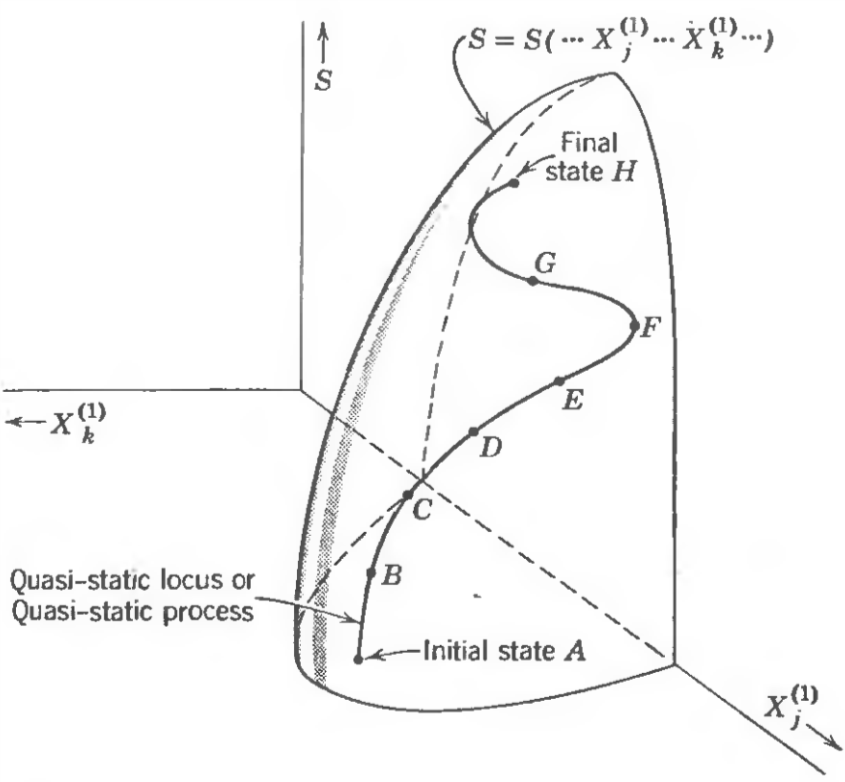
\includegraphics[width=.8\textwidth]{Pictures/fig4.3.png}
\figcaption{一个准静态过程在热力学构形空间中的表示。}
\label{fig4.3}
\end{figure}

{\it $P\,\mathrm dV$作为机械功以及$T\,\mathrm dS$作为热交换的定义仅对准静态过程成立。}

考虑一个{\it 封闭}系统,经历一系列状态$A,B,C,\dots ,H$,近似于一条准静态轨迹。这个系统能在移除一些内部约束后从$A$到$B$。封闭系统能到达$B$当且仅当$B$态在所有可达到的态中有最大的熵值。这里即$B$态的熵比$A$态要高。因此,封闭系统中从$A$态到$B$态的过程是有方向性的。它从一个熵低的态,$A$,到达一个熵高的态$B$,没法倒过来。这样一个过程是{\it 不可逆的(irreversible)}。

{\it 封闭系统的一条准静态轨迹可以由一条实际轨迹近似,仅当轨迹上熵值单调不减。}

{\it 熵增为零的准静态过程被称为可逆过程(reversible process)}(图\ref{fig4.4})。这类过程末态的熵与初态相等,其可以依两个方向移动。

\begin{figure}
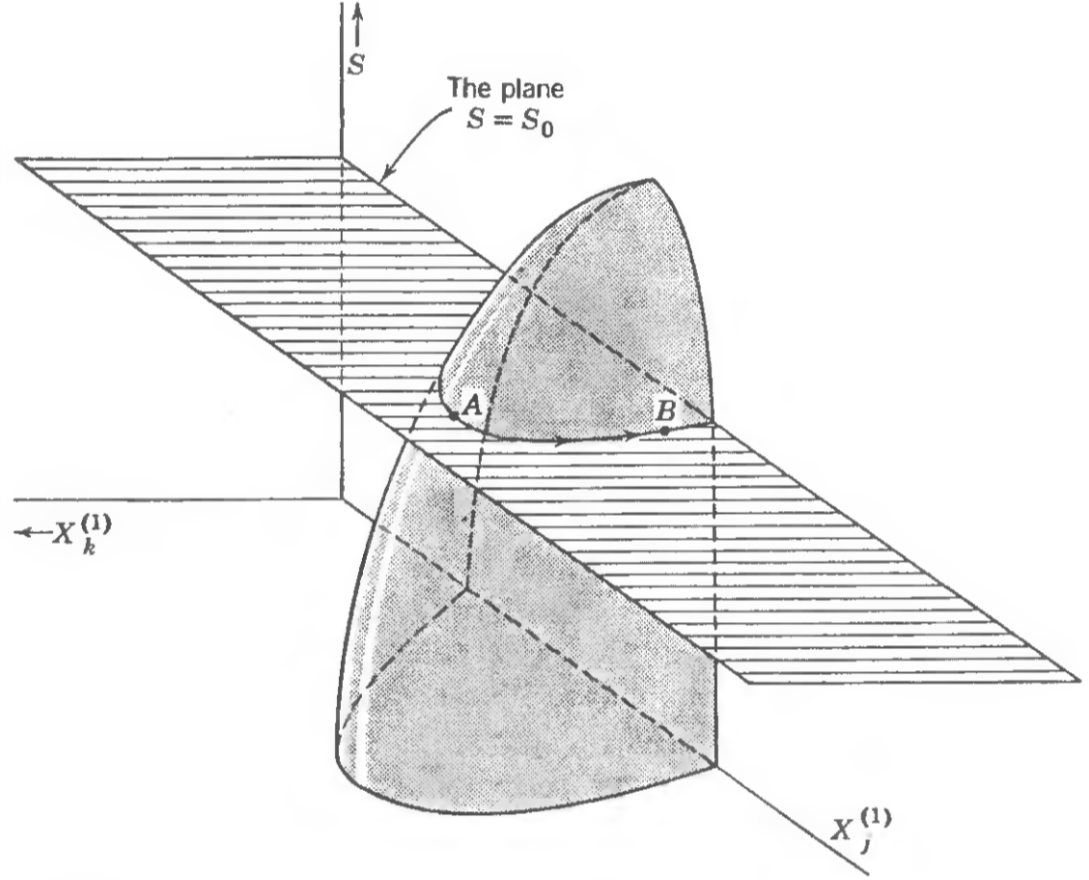
\includegraphics[width=.8\textwidth]{Pictures/fig4.4.png}
\figcaption{沿着等熵线的可逆过程}
\label{fig4.4}
\end{figure}

\subsection*{习题}
\begin{itemize}
\item[4.2-1] 每个可逆过程是否都对应于一条准静态轨迹?每条准静态轨迹是否都对应于一个可逆过程?对于从$A$态到$H$态的任意实际过程,是否存在一些有着同样的两个末态$A$和$H$的准静态过程?是否存在一些有着同样的两个末态$A$和$H$的可逆过程?
\item[4.2-2] 考虑带有活塞的圆柱中的单原子理想气体。圆柱的壁和活塞都是绝热的。系统初始处于平衡态,但外界的压强在缓慢减小。气体的能量由体积膨胀$\mathrm dV$造成的改变为$\mathrm dU=-P\,\mathrm dV$。证明,利用\eqref{equ3.34}式,有$\mathrm dS=0$,即准静态绝热膨胀是等熵且可逆的。
\item[4.2-3] 单原子理想气体由$V$自由膨胀至$V+\mathrm dV$(回忆习题3.4-8)。证明
\[
\mathrm dS = \frac{NR}{V}\mathrm dV
\]
通过这样一系列无穷小自由膨胀,从$V_i$到$V_f$,证明
\[
\Delta S = NR\ln(\frac{V_f}{V_i})
\]
讨论这种非典型(并且臭名昭著的)“连续自由膨胀”过程是否为准静态过程需要一些精细的考虑。作为正面因素,无穷小膨胀的末态可以在轨迹上作到%
\mpar{与初态}%
充分的接近。而作为负面因素,在实现上,系统在每次膨胀中必须经历非平衡态;微膨胀的不可逆性是本质的和不可约的。$\mathrm dS>0$和$\mathrm dQ=0$的事实与对所有准静态过程的假设$\mathrm dQ=T\mathrm dS$相冲突。我们{\it 定义}(某种意义上是循环论证!)连续自由膨胀过程是“本质不可逆的”以及{\it 非准静态的(non-quasi-static)}%
\mpar{另一种解释是,单次自由膨胀这个问题中,外界给原系统添加了另一个子系统——尽管没有能量、粒子数交换。} %
。
\item[4.2-4] 在所考虑的温度范围内,某系统遵循如下方程
\[
T=Av^2/s, \quad P=-2Av\ln(s/s_0)
\]
其中$A$为正常数。这个系统从$v_0$自由膨胀至$v_f$($v_f>v_0$)。求体系的末温$T_f$关于初温$T_0$,以及$v_0,v_f$的函数。求摩尔熵的增量。
\end{itemize}